\documentclass[runningheads]{llncs}
\usepackage[T1]{fontenc}
\usepackage{graphicx}
\graphicspath{{figures/}{report/figures/}{../report/figures/}}
\usepackage{booktabs}
\usepackage{amsmath,amssymb}
\usepackage{tabularx}
\usepackage{cite}
\usepackage{microtype}
\usepackage[hidelinks]{hyperref}
\urlstyle{same}
\usepackage[table,xcdraw]{xcolor}
\usepackage{float}
\usepackage[section]{placeins}

\setlength{\intextsep}{5pt plus 1pt minus 1pt}
\setlength{\textfloatsep}{6pt plus 1pt minus 1pt}
\setlength{\floatsep}{5pt plus 1pt minus 1pt}
\setlength{\abovecaptionskip}{3pt}
\setlength{\belowcaptionskip}{0pt}

\clubpenalty=10000
\widowpenalty=10000
\displaywidowpenalty=10000

\begin{document}
\raggedbottom

\title{Predicting Subjective Readiness in Sports Participants with Personalized Baselines and Explainable AI}
\titlerunning{Predicting Subjective Readiness in Sports Participants}

\author{Minh-Triet Nguyen\inst{1}\orcidID{0009-0006-0519-9479} \and
Phuc Thien Trinh\inst{1}\orcidID{0009-0005-6156-0313} \and
Hung Nguyen Trong\inst{1}\orcidID{0009-0002-9448-3041} \and
Thu Le\inst{1}}

\authorrunning{M.-T. Nguyen et al.}

\institute{FPT University, Ho Chi Minh City, Viet Nam\\
\email{\{trietnguyen0407,tthienphuc32,tronghungnguyen1104\}@gmail.com, thulvm@fpt.edu.vn}}

\maketitle

\begin{abstract}
Forecasting daily athletic readiness provides practitioners with actionable lead time to adjust training loads and prevent overreaching. We evaluate the PMData cohort across 16 recreationally active adult participants over 152 observation days (2,178 participant-days), integrating continuous Fitbit Versa 2 telemetry, PMSys wellness self-reports, and Session-RPE logs under strict causal alignment. Benchmarking ten supervised learning algorithms on within-subject chronological 70/30 splits shows that Extra Trees achieves the lowest holdout error (MAE = 0.982 vs. 1.082 persistence on 404 holdout transitions, a 9.25\% reduction representing an empirical upper bound subject to holdout selection). Feature attribution via TreeSHAP reveals that expanding personal baselines serve as primary predictive anchors (accounting for approximately one-third of top-ten attribution mass, 33.1\%), balanced by wearable biometrics (collectively 33.1\% across five sensor modalities), with progressive feature deletion confirming genuine estimator reliance. Under 16-fold Leave-One-Person-Out (LOPO) cross-validation across all 1,324 transitions, expanding baselines reduce generic error from 1.395 to 1.247, improving predictions for 13 of 16 participants ($p = 0.021$). While cohort persistence remains superior across all 16 participants (mean MAE 1.108) due to tree shrinkage toward the cohort mean (4.91) and extreme set-point outliers, pre-deployment screening during calibration isolates 13 regular athletic participants where personalized machine learning achieves lower average error than persistence (1.171 vs. 1.212). These results demonstrate that cross-subject transfer cannot universally replace within-subject tracking, but pre-deployment calibration successfully identifies athletes who benefit from algorithmic forecasting.

\keywords{Sports analytics \and Machine learning \and Wearable sensors \and Explainable AI \and Subjective readiness \and Leave-One-Person-Out}
\end{abstract}

\section{Introduction}
Monitoring athletic well-being and managing physical training loads are foundational pillars of modern sports science. A participant's daily subjective readiness reflects their holistic capacity to absorb exercise stress, optimize training adaptation, and mitigate overuse injury risk~\cite{bourdon2017,drew2016}. Because readiness emerges from non-linear interactions among prior exercise volume, autonomic recovery, sleep architecture, and perceived muscle soreness~\cite{halson2014,saw2016}, prospective forecasting presents an individualized challenge. Traditional heuristic markers such as Session Rating of Perceived Exertion (Session-RPE)~\cite{foster2001} or the Acute:Chronic Workload Ratio (ACWR)~\cite{gabbett2016} often fail to accommodate biological adaptability and subjective rating scales~\cite{windt2017}. Modern commercial wearables capture continuous physiological telemetry (resting heart rate, active calories, sleep stages)~\cite{seshadri2019} alongside daily mobile wellness surveys (PMSys)~\cite{thambawita2020pmdata}. However, sports analytics research frequently suffers from temporal data leakage in random splits violating causality~\cite{kapoor2023}, unverified XAI attributions lacking empirical faithfulness testing~\cite{guidotti2018,hooker2019}, and reporting scale shifts degrading cross-subject generalization.

To address these vulnerabilities, we establish a leakage-aware forecasting framework using the PMData collection across 16 participants over 152 observation days (2,178 recorded participant-days)~\cite{thambawita2020pmdata}. We engineer 22 causal predictors strictly from past-only history ($X_{\leq t}$) on a continuous calendar grid, forming 1,324 valid transition pairs ($t \to t+1$) with train-only median imputation. Under within-subject chronological 70/30 partitioning (920 training transitions, 404 holdout test transitions), Extra Trees achieves superior forecasting skill (MAE = 0.982, $R^2 = 0.400$), reducing prediction error by 9.25\% over persistence (1.082). Through progressive feature deletion without retraining, we confirm the predictive importance of personal baselines alongside wearable biometrics. In 16-fold Leave-One-Person-Out (LOPO) cross-validation, expanding baselines reduce mean participant MAE from 1.395 to 1.247, improving error in 13 of 16 participants (two-tailed binomial sign test across participants: $p = 0.021$). However, both cross-subject models remain inferior to within-subject persistence (1.108), with personalized models outperforming persistence in 7 of 16 participants (generic models in only 3 of 16), highlighting the challenge of cross-subject generalizability.

\section{Related Work}
Predictive sports analytics increasingly prioritizes prospective decision support~\cite{novatchkov2013,claudino2019}, where subjective wellness surveys detect acute fatigue earlier than mechanical load metrics~\cite{saw2016,bourdon2017}. To balance bias and variance across complex physiological interactions~\cite{bzdok2018}, existing studies deploy tree ensembles, support vector machines, and neural networks~\cite{carey2018,rossi2018}, augmented by nocturnal resting heart rate (RHR) and sleep stages as objective recovery markers~\cite{buchheit2014,seshadri2019}. However, evaluating models on randomly shuffled records obscures performance degradation when predicting prospectively or across individuals. Furthermore, while non-linear models offer high predictive accuracy, their black-box structures impede coaching adoption~\cite{shmueli2010,molnar2020}. Post-hoc explainers such as KernelSHAP~\cite{lundberg2017}, TreeSHAP~\cite{lundberg2020trees}, and LIME~\cite{ribeiro2016} attribute feature importance, but explainers can disagree or misrepresent actual dependencies~\cite{guidotti2018}. Inspired by Remove and Retrain (ROAR)~\cite{hooker2019}, we develop an empirical feature deletion protocol without retraining to measure degradation curves across multiple explainer families, providing verifiable evidence of estimator reliance.

\section{Methodology and Experimental Setup}
We propose an integrated workflow unifying multi-modal telemetry ingestion, leakage-aware causal preprocessing, and three structured evaluation tracks. We depict our end-to-end analytical pipeline in Fig.~\ref{fig:pipeline}.

\begin{figure}[H]
\centering
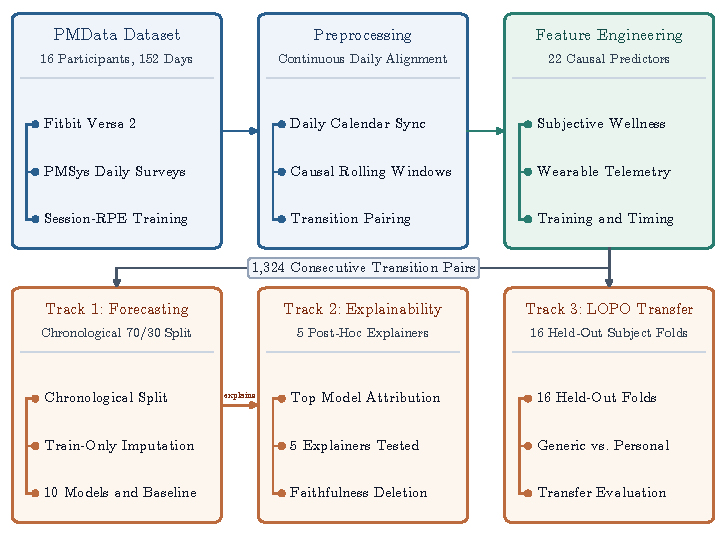
\includegraphics[width=0.88\linewidth]{fig_pipeline.pdf}
\caption{End-to-end analytical pipeline spanning multi-modal data ingestion (Stage~1), causal preprocessing (Stage~2), feature engineering (Stage~3), and three-track evaluation (Stage~4).}
\label{fig:pipeline}
\end{figure}

In Fig.~\ref{fig:pipeline}, we outline the four core stages of our framework. Specifically, Stage~1 ingests three multi-modal streams across 16 recreationally active participants over 152 observation days (2,178 recorded participant-days), encompassing continuous Fitbit Versa 2 telemetry (resting heart rate, daily step volume, active minutes, and multi-stage sleep architecture), daily PMSys mobile wellness surveys (capturing subjective readiness $y_{i,t} \in [0, 10]$ alongside fatigue, mood, muscle soreness, and stress), and Session-RPE training logs (quantifying daily exertion via duration and perceived exertion ratings); Stage~2 performs causal preprocessing by synchronizing modalities on a continuous daily calendar grid to prevent temporal leakage, filtering consecutive transitions to yield 1,324 valid pairs ($t \to t+1$); Stage~3 engineers 22 causal predictors across subjective wellness, wearable biometrics, and training workload modalities (incorporating acute-to-chronic workload ratios and personalized baseline calibrations $\mu_{i,t}^{\text{ready}}$ and $\Delta y_{i,t}$), imputing missing values strictly using training-partition medians; and Stage~4 coordinates a three-track evaluation framework: Track~1 benchmarks ten supervised machine learning algorithms across six model families against persistence under a within-subject chronological 70/30 split (the first 70\% of transitions per participant for training, totaling 920 pairs; the remaining 30\% for holdout testing, totaling 404 pairs); Track~2 evaluates attribution faithfulness across five post-hoc explainers via progressive feature deletion without model retraining; and Track~3 assesses cross-subject generalizability across all 1,324 transitions using 16-fold Leave-One-Person-Out (LOPO) cross-validation.

\subsection{Cohort Ingestion and Causal Feature Engineering}
We evaluate the open-access PMData collection~\cite{thambawita2020pmdata}, tracking 16 adult participants (13 male, 3 female; aged 23--60 years, mean $34.9 \pm 11.7$) over 152 days (2019-11-01 to 2020-03-31, 2,178 participant-days). Streams combine continuous Fitbit Versa 2 telemetry (steps on 2,107 days, 3.3\% missingness), daily PMSys wellness surveys (0--10 scale, 1,668 surveys, 23.4\% missingness), and Session-RPE logs ($\text{duration} \times \text{RPE}$ using PMSys perceived exertion). Requiring consecutive logs and $\geq 7$ days of prior context on a continuous calendar grid yields 1,324 complete transition pairs ($t \to t+1$) across all 16 subjects, with train-only median imputation.

To capture readiness determinants without temporal leakage, we engineer 22 causal predictors ($X_{\leq t}$) across four groups: wearable telemetry (9 features: steps, active minutes, sedentary duration, nocturnal RHR, sleep duration, sleep efficiency, 7-day rolling sleep, RHR deviation $\text{RHR}_t - \mu_{\text{RHR},i,t}$, step deviation); subjective wellness (8 features: fatigue, mood, prior-day readiness $y_t$, sleep quality, soreness, stress, expanding baseline $\mu_{i,t}^{\text{ready}}$, deviation $\Delta y_{i,t}$); training workload (4 features: daily load $\text{sRPE}$, acute 7-day load, chronic 28-day load, ACWR); and calendar day-of-week. All rolling windows are calculated on the continuous calendar grid prior to transition pairing, ensuring strict causal alignment. Participant readiness means range from 2.78 to 7.36 across individuals (unweighted mean $\mu = 5.03 \pm 1.25$, pooled transition mean 4.91 across 1,324 pairs, raw survey mean 4.94; discrete integer range 1--10).

\subsection{Problem Formulation and Evaluation Framework}
We formulate next-day readiness forecasting as follows: let $y_{i,t} \in [0, 10]$ denote participant $i$'s reported readiness on day $t$. We aim to forecast next-day readiness $\widehat{y}_{i,t+1} = f(X_{i,\leq t})$ using past-only feature history available up to evening $t$. Because readiness exhibits autocorrelation, we establish a within-subject persistence baseline $\widehat{y}_{i,t+1}^{\text{persist}} = y_{i,t}$, representing the heuristic assumption that tomorrow's readiness mirrors today's (achieving $\text{MAE} = 1.082$ on the 404 holdout transitions and 1.108 across all 1,324 transitions). A machine learning model must outperform persistence to demonstrate prospective utility.

In Track~1, we benchmark ten supervised machine learning algorithms across six families against persistence under a within-subject chronological 70/30 split (the first 70\% of chronological transitions per participant are assigned to training, totaling 920 transitions; the remaining 30\% form the holdout test set, totaling 404 transitions): regularized linear models (Ridge, Elastic Net), $k$-NN, CART, randomized tree ensembles (Random Forest~\cite{breiman2001}, Extra Trees~\cite{geurts2006}), gradient boosted trees (HistGB, LightGBM~\cite{ke2017}, XGBoost~\cite{chen2016}), and an MLP neural network. Comparing ten algorithms identifies the top-performing estimator family, though reporting the minimum test error without nested cross-validation represents an empirical upper bound. This directly motivates Track~3, where 16-fold Leave-One-Person-Out (LOPO) cross-validation evaluates zero-shot transfer across all 1,324 transitions without holdout selection.

In Track~2, we evaluate attribution reliability across five explainers: TreeSHAP~\cite{lundberg2020trees}, KernelSHAP~\cite{lundberg2017} (50 background samples), LIME~\cite{ribeiro2016} (1,000 perturbations), Permutation Importance~\cite{breiman2001}, and Tree Gain, applied to the gradient-boosted tree ensemble (LightGBM). Following progressive feature deletion without model retraining~\cite{hooker2019}, we sequentially replace top $k \in \{1, \dots, 20\}$ features with training-set medians (averaged over 20 Monte Carlo runs for random deletion). We measure faithfulness via Deletion Area ($\mathrm{AUC}_{\text{deletion}} = \frac{1}{K}\sum_{k=1}^K \mathrm{MAE}(k)$), top-5 degradation, runtime, and bootstrap rank stability across 50 resamples.

In Track~3, to address individual rating scale differences, we compute expanding readiness baselines for $t \geq 2$ as $\mu_{i,t}^{\text{ready}} = \frac{1}{t-1} \sum_{j=1}^{t-1} y_{i,j}$ (training-set median for $t=1$) and deviations $\Delta y_{i,t} = y_{i,t} - \mu_{i,t}^{\text{ready}}$. Under 16-fold Leave-One-Person-Out (LOPO) cross-validation with gradient-boosted trees (LightGBM), Generic models train on 15 participants without baseline features, whereas Personalized models incorporate the held-out subject's expanding baselines from days $1 \dots t-1$. Evaluation spans all 1,324 complete transitions, reporting unweighted mean participant MAE ($\frac{1}{16}\sum_i \text{MAE}_i$) and pooled prediction MAE ($\frac{1}{N}\sum_i \sum_t |y_{i,t+1} - \widehat{y}_{i,t+1}|$). Pipelines were implemented in Python 3.10 using scikit-learn 1.4, xgboost 2.0, lightgbm 4.3, and shap 0.44.

\section{Results}

\subsection{Readiness and Training Load Dynamics}
Bivariate analysis of 1,648 single-day records shows that days following hard training ($\text{sRPE} > 300$, mean 5.24, $n=201$) exhibit slightly higher next-day readiness than rest days ($\text{sRPE} = 0$, mean 4.92, $n=1066$) or light training ($0 < \text{sRPE} \leq 300$, mean 4.83, $n=381$), alongside longer sleep (436.9 vs. 404.2 min). Because this observation lacks causal controls, workout self-selection remains unverified.

\subsection{Multi-Model Predictive Accuracy}
We benchmark ten supervised machine learning algorithms across six distinct model families against persistence under strict chronological within-subject train-test splits (920 training transitions, 404 holdout test transitions). We summarize the resulting test performance on the 30\% temporal holdout in Table~\ref{tab:models_results}.

\begin{table}[H]
\centering
\caption{Multi-model predictive accuracy evaluation comparing ten supervised learning algorithms against within-subject persistence on the 30\% temporal holdout (404 transitions across 16 participants). Bold denotes optimal performance across evaluation criteria.}
\label{tab:models_results}
\begingroup\small\setlength{\tabcolsep}{3.5pt}
\begin{tabular*}{\linewidth}{@{\extracolsep{\fill}}lrrrrr}
\toprule
Model & MAE $\downarrow$ & RMSE $\downarrow$ & $R^2$ $\uparrow$ & \shortstack{MAE seed\\SD $\downarrow$} & \shortstack{Fit (s)\\$\downarrow$}\\
\midrule
Persistence & 1.082 & 1.578 & 0.092 & 0.00000 & 0.000\\
Ridge & 1.056 & 1.351 & 0.334 & 0.00000 & 0.003\\
Elastic Net & 1.049 & 1.345 & 0.340 & 0.00000 & 0.003\\
$k$-NN & 1.073 & 1.405 & 0.280 & 0.00000 & 0.002\\
Decision Tree & 1.215 & 1.554 & 0.120 & 0.00003 & 0.006\\
Random Forest & 1.018 & 1.319 & 0.366 & 0.00315 & 0.774\\
Extra Trees & \textbf{0.982} & \textbf{1.283} & \textbf{0.400} & 0.00164 & 0.586\\
HistGB & 1.139 & 1.462 & 0.221 & 0.00000 & 2.892\\
LightGBM & 1.114 & 1.427 & 0.258 & 0.00805 & 1.326\\
XGBoost & 1.071 & 1.383 & 0.302 & 0.00765 & 2.087\\
Small MLP & 1.221 & 1.848 & -0.247 & 0.02220 & 0.651\\
\bottomrule
\end{tabular*}\endgroup
\end{table}

In Table~\ref{tab:models_results}, Extra Trees achieves superior forecasting across all primary metrics: the lowest test MAE (0.982), lowest RMSE (1.283), and highest $R^2$ (0.400), reducing prediction error by 9.25\% over within-subject persistence (1.082). Random Forest (1.018), Elastic Net (1.049), Ridge (1.056), XGBoost (1.071), and $k$-NN (1.073) also outperform persistence, whereas gradient-boosted variants (HistGB: 1.139; LightGBM: 1.114), single Decision Trees (1.215), and Small MLP (1.221) underperform the reference. Because Extra Trees was selected among ten algorithms on the holdout, this 9.25\% gain represents an empirical upper bound subject to selection bias. A 1,000-sample participant-clustered bootstrap on test predictions yields a 95\% confidence interval of [0.807, 1.166] for Extra Trees MAE and an error reduction over Random Forest of +0.035 (95\% clustered CI: [0.002, 0.072]; Extra Trees superior in 98.2\% of bootstrap resamples).

\subsection{Explainability Sensitivity Evaluation}
To evaluate whether feature attributions reflect true estimator dependencies, we execute progressive feature neutralization across five explainer frameworks. We report the quantitative degradation profiles under progressive feature deletion in Table~\ref{tab:explainers}.

\begin{table}[H]
\centering
\caption{Faithfulness benchmark comparing five post-hoc explainer frameworks under progressive feature neutralization without model retraining. Bold marks optimal metric performance across criteria; n/a denotes not applicable.}
\label{tab:explainers}
\begingroup\small\setlength{\tabcolsep}{3.5pt}
\begin{tabular*}{\linewidth}{@{\extracolsep{\fill}}lrrrr}
\toprule
Method & \shortstack{MAE after\\top-5 $\uparrow$} & \shortstack{Deletion\\Area $\uparrow$} & \shortstack{Rank\\stability $\uparrow$} & \shortstack{Time (s)\\$\downarrow$}\\
\midrule
Full model (no deletion) & 1.114 & n/a & n/a & n/a\\
Gain & 1.310 & 1.285 & \textbf{0.880} & \textbf{0.002}\\
KernelSHAP & 1.353 & 1.313 & 0.736 & 8.624\\
LIME & \textbf{1.355} & 1.310 & 0.809 & 0.744\\
Permutation & 1.330 & \textbf{1.322} & 0.774 & 0.909\\
TreeSHAP & 1.318 & 1.307 & 0.808 & 1.231\\
Random deletion & 1.133 & 1.158 & n/a & n/a\\
\bottomrule
\end{tabular*}\endgroup
\end{table}

From the deletion profiles in Table~\ref{tab:explainers}, we find that neutralizing the top-5 features degrades the baseline model MAE from 1.114 to 1.310--1.355 across all five explainers ($\approx 20\%$ error inflation), substantially outpacing random deletion (1.133) and confirming that all explainers capture genuine predictive drivers. Differences across explainers are narrow (Deletion Area 1.285--1.322): Permutation Importance achieves the highest Deletion Area (1.322), while Tree Gain delivers optimal rank stability (0.880) with near-instant runtime (0.002~s). Error escalates rapidly across the initial 5 features, confirming that predictive reliance concentrates on a compact core of dominant predictors (mapped via TreeSHAP in Fig.~\ref{fig:shap}).

\begin{figure}[H]
\centering
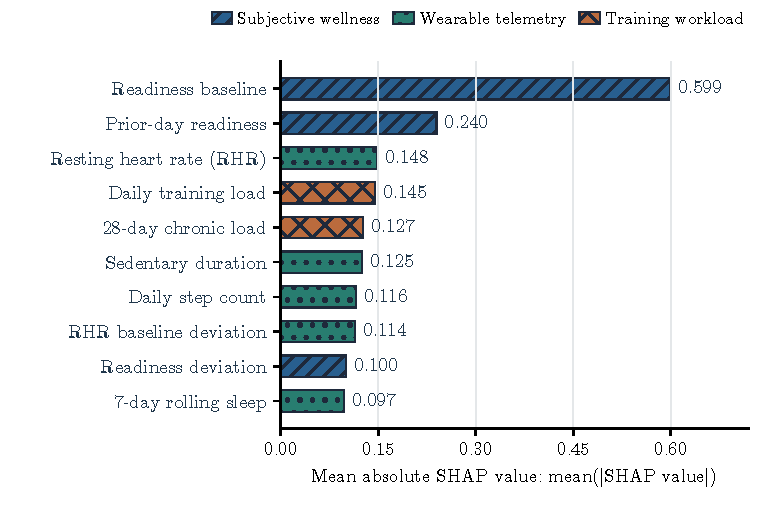
\includegraphics[width=0.58\linewidth]{fig_shap.pdf}
\caption{Global TreeSHAP feature importance across the top ten predictors, distinguished by hatch pattern and shading per feature modality. Expanding readiness baseline provides the primary predictive anchor, complemented by prior-day readiness and wearable biometrics.}
\label{fig:shap}
\end{figure}

In Fig.~\ref{fig:shap}, expanding baseline readiness (mean $|\text{SHAP}| = 0.599$, 33.1\% of top-ten mass) and prior-day readiness (0.240, 13.2\%) emerge as primary anchors. Wearable biometrics account for 33.1\% of attribution mass (0.600 across nocturnal RHR, sedentary duration, steps, RHR deviation, rolling sleep), Session-RPE training features contribute 15.0\% (0.272 across daily and chronic load), and subjective wellness features total 51.9\%. Thus, baselines calibrate personal set-points while wearable biometrics capture daily physiological context.

\subsection{Personalization and LOPO Validation}
We evaluate cross-subject generalizability using Leave-One-Person-Out (LOPO) cross-validation across all 16 held-out participants using gradient-boosted trees (LightGBM). In Table~\ref{tab:lopo_full}, we contrast per-participant forecasting errors against individual baseline statistics.

\begin{table}[H]
\centering
\caption{Leave-One-Person-Out (LOPO) cross-validation errors across all 16 participants (1,324 transitions), contrasting individual baseline statistics with within-subject persistence, generic, and personalized gradient-boosted tree models (LightGBM). Bold in Personalized MAE marks participants where personalized ML outperforms persistence (7 of 16); bold in MAE Reduction marks participants improved over generic ML (13 of 16).}
\label{tab:lopo_full}
\begingroup\footnotesize\setlength{\tabcolsep}{2.8pt}\renewcommand{\arraystretch}{0.95}
\begin{tabular*}{\linewidth}{@{\extracolsep{\fill}}lrrrrrrrr}
\toprule
ID & $N$ & $\mu$ & $\sigma$ & Adh. & \shortstack{MAE\\Persist} & \shortstack{MAE\\Generic} & \shortstack{MAE\\Person} & \shortstack{MAE\\Reduc.}\\
\midrule
p01 & 120 & 6.22 & 1.41 & 91\% & 1.367 & 1.461 & \textbf{1.110} & \textbf{+0.351}\\
p02 & 55 & 4.77 & 1.28 & 65\% & 0.873 & 1.072 & 1.265 & -0.193\\
p03 & 30 & 5.00 & 0.18 & 43\% & 0.000 & 0.397 & 0.269 & \textbf{+0.128}\\
p04 & 124 & 5.19 & 1.04 & 91\% & 1.089 & 1.110 & \textbf{0.925} & \textbf{+0.186}\\
p05 & 106 & 2.78 & 2.49 & 84\% & 0.255 & 2.357 & 2.403 & -0.045\\
p06 & 137 & 4.79 & 1.73 & 97\% & 1.766 & 1.504 & \textbf{1.437} & \textbf{+0.068}\\
p07 & 115 & 3.64 & 1.23 & 87\% & 1.165 & 1.345 & 1.276 & \textbf{+0.068}\\
p08 & 71 & 4.82 & 1.81 & 66\% & 1.310 & 1.413 & 1.422 & -0.009\\
p09 & 79 & 4.71 & 0.99 & 66\% & 0.823 & 0.970 & 0.870 & \textbf{+0.100}\\
p10 & 82 & 3.40 & 1.40 & 62\% & 1.354 & 1.611 & \textbf{1.235} & \textbf{+0.376}\\
p11 & 95 & 5.33 & 1.49 & 70\% & 1.137 & 1.195 & 1.141 & \textbf{+0.054}\\
p12 & 51 & 5.32 & 1.75 & 49\% & 1.725 & 1.481 & \textbf{1.416} & \textbf{+0.066}\\
p13 & 23 & 7.36 & 2.43 & 32\% & 1.717 & 2.234 & 2.061 & \textbf{+0.173}\\
p14 & 103 & 6.53 & 0.89 & 79\% & 0.563 & 1.460 & 0.830 & \textbf{+0.630}\\
p15 & 71 & 6.47 & 1.94 & 61\% & 1.958 & 2.129 & \textbf{1.798} & \textbf{+0.331}\\
p16 & 62 & 4.13 & 0.60 & 54\% & 0.629 & 0.574 & \textbf{0.501} & \textbf{+0.073}\\
\midrule
Mean ($N=16$) & 83 & 5.03 & 1.42 & 69\% & 1.108 & 1.395 & 1.247 & \textbf{+0.147}\\
Subgroup ($N=13$) & 90 & 5.03 & 1.35 & 72\% & 1.212 & 1.333 & \textbf{1.171} & \textbf{+0.162}\\
Pooled & 1,324 & 4.91 & -- & -- & 1.126 & 1.421 & 1.259 & \textbf{+0.162}\\
\bottomrule
\end{tabular*}\endgroup
\end{table}

In Table~\ref{tab:lopo_full}, we report per-participant LOPO performance alongside baseline statistics ($\mu$, $\sigma$, and adherence across 1,668 raw surveys, cohort mean $\mu = 5.03$; transition weighted mean = 4.91). Across all 16 participants, cohort persistence achieves $\text{MAE} = 1.108$, outperforming generic (1.395) and personalized (1.247) models due to tree shrinkage toward the cohort mean (4.91). However, persistence is heavily anchored by p03, whose near-zero variance ($\sigma = 0.18$, 30 transitions, 43\% adherence) yields $\text{MAE} = 0.000$; excluding p03 raises cohort persistence error to 1.182 (vs. 1.313 for personalized ML). Signed prediction bias confirms severe shrinkage on extreme outliers: the generic model overpredicts for p05 ($\mu = 2.78$, bias = $+2.34$) and underpredicts for p13 ($\mu = 7.36$, bias = $-2.18$), driving a strong correlation between cohort distance $|\mu_i - 4.91|$ and generic MAE ($r = 0.744$, $p = 0.001$; Spearman $\rho = 0.662$, $p = 0.005$). While expanding baselines mitigate shrinkage for moderate deviations (reducing MAE in 13 of 16 subjects, $p = 0.021$; $r = 0.777$, $p = 0.001$ on 14 non-extreme subjects), decision trees cannot extrapolate for extreme set-points. Crucially, excluding the three boundary cases (p03, p05, p13) reverses the error ranking: on the remaining 13 participants, personalized ML achieves lower mean error than persistence (1.171 vs. 1.212, Subgroup row in Table~\ref{tab:lopo_full}). Across subjects, personalized ML beats persistence in 7 of 13 ($p = 1.000$, sign test), achieving superior average accuracy on regular athletic responders.

To profile participant-level heterogeneity and response archetypes, Fig.~\ref{fig:athlete_profiles} illustrates the cohort LOPO ranking and archetype comparisons.

\begin{figure}[H]
\centering
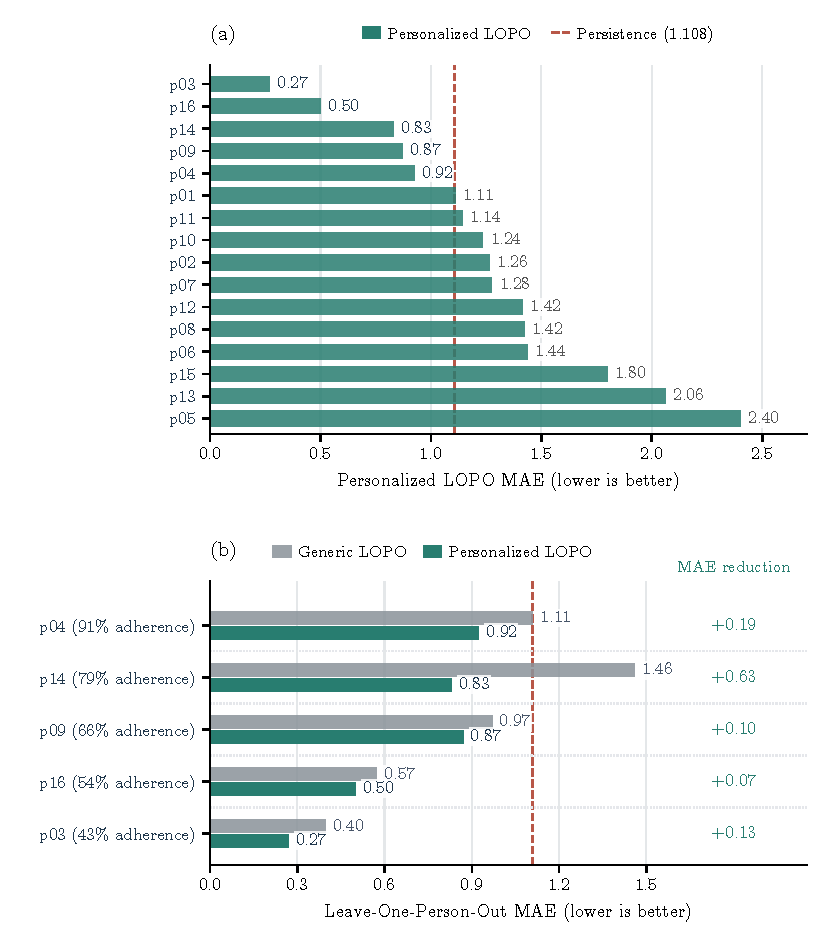
\includegraphics[width=0.55\linewidth]{fig_athlete_profiles.pdf}
\caption{Cohort-wide Leave-One-Person-Out (LOPO) cross-validation: (a) 16-participant personalized MAE ranking; (b) Selected archetype comparisons between generic and personalized errors. Dashed vertical line marks cohort persistence error (1.108); percentages denote survey reporting adherence.}
\label{fig:athlete_profiles}
\end{figure}

In Fig.~\ref{fig:athlete_profiles}(a), personalized errors span from 0.27 to 2.40 across individuals. For low-variance participants (p03: $\sigma = 0.18$), persistence provides an unbeatable heuristic ($\text{MAE} = 0.000$). In Fig.~\ref{fig:athlete_profiles}(b), archetype comparisons show that for subjects with pronounced set-point offsets (p14: $\mu = 6.53$), personalization delivers substantial error reduction (+0.630), though within-subject persistence remains competitive (0.563).

\section{Discussion}
Our findings highlight three key insights for applied sports analytics. First, prospective readiness forecasting requires individual baseline calibration rather than telemetry alone; subjective readiness reflects personal perceptual scales that vary widely across individuals. Second, tree ensemble shrinkage creates a structural barrier for zero-shot transfer: models pull predictions toward the cohort mean (4.91), penalizing subjects with extreme set-points. Because decision trees perform piecewise-constant regression and cannot extrapolate beyond training label ranges, personal baselines counteract shrinkage for moderate offsets ($r = 0.777$, $p = 0.001$ across 14 non-extreme subjects; error reduced in 13 of 16, sign test $p = 0.021$), but provide minimal relief for extreme outliers (p05, p13). Third, sports readiness systems should integrate an actionable pre-deployment screening rule during initial calibration: if baseline rating variance $\sigma_i < 0.5$ (e.g., p03) or cohort offset $|\mu_i - 4.91| > 2.0$ (e.g., p05, p13), within-subject persistence serves as the optimal heuristic; for all remaining athletes ($N=13$), personalized ML achieves superior average accuracy over persistence (1.171 vs. 1.212) alongside actionable biometric explanations.

Methodologically, our study carries several limitations. First, our evaluation lacks full modality ablation beyond baseline anchors and omits specialized time-series baselines (e.g., autoregressive AR or EMA models). Second, Track~2 median neutralization may induce out-of-distribution feature combinations during progressive deletion, while commercial Fitbit telemetry carries inherent sensor noise and motion artifacts. Third, Track~1 holdout selection lacks nested cross-validation, while Track~3 LOPO omits cross-subject temporal blocking, leaving calendar confounding unadjusted. Finally, PMData represents an observational single cohort of 16 participants during early 2020 COVID-19 restrictions with 23.4\% survey non-response, and archetypes were identified post-hoc. Future work will evaluate deep sequential architectures across multi-cohort populations with prospective coaching trials.

\section{Conclusion}
We established a leakage-aware readiness forecasting framework using PMData across 16 participants over 152 days. Chronological benchmarking showed that Extra Trees achieved the lowest error (MAE = 0.982, $R^2 = 0.400$), reducing MAE by 9.25\% over persistence on the temporal holdout as an empirical upper bound. Feature attribution and progressive deletion confirmed that personal baselines serve as primary predictive anchors, complemented by wearable biometrics. Under LOPO cross-validation, expanding baselines reduced error over generic models in 13 of 16 participants ($1.395 \to 1.247$, sign test $p = 0.021$). While cohort persistence remained superior across all 16 subjects (1.108 vs. 1.247) due to outlier distortion, excluding the three boundary cases (p03, p05, p13) reversed the ranking, with personalized ML outperforming persistence (1.171 vs. 1.212) on the remaining 13 participants. These findings demonstrate that prospective readiness forecasting requires individualized calibration, where pre-deployment screening identifies candidates who benefit from algorithmic guidance.

\clearpage
\begingroup
\renewcommand{\textbf}[1]{#1}
\small
\let\oldthebibliography\thebibliography
\renewcommand{\thebibliography}[1]{%
  \oldthebibliography{#1}%
  \setlength{\itemsep}{0pt plus 0.2pt}%
  \setlength{\parskip}{0pt}%
}
\bibliographystyle{splncs04}
\bibliography{references}
\endgroup

\end{document}
